Dengue fever is the most important arboviral disease world-wide, with \Aea\ being the major vector.
Interactions between the mosquito host and dengue viruses (\gls{DENV}) are complex and vector competence varies among geographically-distinct \Aa\ populations.
Additionally, dengue is caused by four antigenically-distinct viral serotypes (\gls{DENV}1–4), each with multiple genotypes.
Each virus genotype interacts differently with vertebrate and invertebrate hosts.
Analyses of alterations in mosquito transcriptional profiles during \gls{DENV} infection are expected to provide the basis for identifying networks of genes involved in responses to viruses and contribute to the molecular-genetic understanding of vector competence.
In addition, this knowledge is anticipated to support the development of novel disease-control strategies.
RNA-seq technology was used to assess genome-wide changes in transcript abundance at 1, 4 and 14 days following \gls{DENV}2 infection in carcasses, midguts and salivary glands of the \Aa\ Chetumal strain.
\gls{DENV}2 affected the expression of 397 \Aa\ genes, most of which were down-regulated by viral infection.
Differential accumulation of transcripts was mainly tissue- and time-specific.
Comparisons of our data with other published reports reveal conservation of functional classes, but limited concordance of specific mosquito genes responsive to \gls{DENV}2 infection.
These results indicate the necessity of additional studies of mosquito-\gls{DENV} interactions, specifically those focused on recently-derived mosquito strains with multiple dengue virus serotypes and genotypes.


\subsection{Introduction}
The World Health Organization lists dengue as the most important arthropod-borne viral disease of humans \cite{WHO2009}.
The major vector of all four dengue virus serotypes (\gls{DENV}1–4) is the cosmopolitan mosquito, \Aea.
Close association with human populations and increasing intercontinental travel favor the expansion of its geographic distribution.
There are no effective prophylactic and therapeutic drugs specific for dengue, and vaccine development is hindered by potential antibody-dependent enhancement that could put people at greater risk of life-threatening, severe dengue \cite{Gubler2002}.
As a consequence, vector control is currently the only practical and effective strategy for disease prevention.
The \Aa\ genome was sequenced and knowledge of genome-wide changes in patterns of gene expression following \gls{DENV} infection is expected to identify genes involved in vector competence, the intrinsic ability of the mosquito to host and transmit \gls{DENV} \cite{Nene2007}, \cite{Kramer2003}.
This knowledge, coupled with germline transformation technology and anti-viral effector molecules, can be applied to the development of genetically-modified mosquitoes incapable of arbovirus transmission \cite{James2007}, \cite{Franz2006}, \cite{Mathur2010}.

Although vertical transmission of dengue viruses has been reported, mosquitoes become infected mainly following ingestion of an infectious-blood meal \cite{Gunther2007}, \cite{Angel2008}.
Viruses are transmitted to new human hosts during a subsequent bloodmeal following an \gls{EIP} of 7–14 days.
The duration of the \gls{EIP} depends on the mosquito strain, virus genotype and environmental factors \cite{Watts1987}, \cite{Black2002}, \cite{Anderson2006}. \cite{Salazar2007}, \cite{Lambrechts2011}.
During the first 1–2 \gls{dpi}, \gls{DENV}s invade midgut epithelial cells through receptor-mediated endocytosis and initiate replication \cite{Bennett2002}, \cite{Heinz2003}, \cite{Rey2003}, \cite{Mercado-Curiel2008}.
These processes involve both viral and host cellular factors \cite{Samsa2009}.
Infection spreads laterally in the midgut epithelium to cells adjacent to those infected originally \cite{Salazar2007}.
Virus titers peak in the midgut usually between 7–10 \gls{dpi} and are followed by a decline \cite{Salazar2007}, \cite{Xi2008}.
\gls{DENV} infection disseminates from the midgut throughout the body, presumably through the tracheal system, reaching the salivary glands as early as 3 \gls{dpi} \cite{Salazar2007}.
Maximum virus titers in the salivary glands are reached 12–18 \gls{dpi}.
The saliva of an infected mosquito containing \gls{DENV}s is injected in a human host during feeding to complete the transmission cycle.

\Aea\ populations of different geographic origin vary in their vector competence.
Phenotypes include those in which \gls{DENV}s either cannot establish a midgut infection (Midgut Infection Barrier) or cannot disseminate to other tissues (Midgut Escape Barrier) \cite{Black2002}, \cite{Gubler1976}, \cite{Cox2011}.
Other phenotypes manifest in the absence of virions in the saliva (Transmission Barrier).
Differences in intensity of infection (peak titers) and duration of \gls{EIP} also are observed among mosquito strains \cite{Salazar2007}.

Multiple quantitative trait loci are associated with MIB and MEB, but specific genes have yet to be identified \cite{Black2002}.
Mosquito genes and physiological pathways related to innate immunity, redox activity, energy production and metabolism are modulated in response to \gls{DENV} infection \cite{Xi2008}, \cite{Sanchez-Vargas2009}, \cite{Sim2010}, \cite{Tchankouo-Nguetcheu2010}, \cite{Luplertlop2011}, \cite{Behura2011}, \cite{Sim2012}, \cite{Colpitts2011}.
These observations come from multiple studies of specific mosquito tissues and time points following infection, and used different combinations of \gls{DENV}2 genotypes and \Aa\ strains.

We investigated genome-wide changes in transcript accumulation in mosquito midguts, carcasses and salivary glands at 1, 4 and 14 \gls{dpi} during the course of \gls{DENV}2 infection.
This analysis was conducted by RNA-seq with the Chetumal (CTM) strain of \Aa\ and \gls{DENV}2-Jam1409.
CTM was colonized recently (2005) from mosquitoes from the Yucatan Peninsula and is well-characterized for its response to non-infectious blood meals and for the kinetics of \gls{DENV}2-Jam1409 infection \cite{Salazar2007}, \cite{Bernhardt2012}, \cite{bonizzoni2012strain}.
A total of 397 genes had transcripts that showed statistically-significant differential accumulation following \gls{DENV} infection, comprising both those found previously and those that are novel to this study, emphasizing the complex interaction between \Aa\ and \gls{DENV}s \cite{Xi2008}, \cite{Sim2010}, \cite{Tchankouo-Nguetcheu2010}, \cite{Luplertlop2011}, \cite{Behura2011}, \cite{Sim2012}, \cite{Colpitts2011}.




\subsection{Results}
\subsubsection{RNA Sequencing and Mapping Summary}

Illumina RNA-seq technology was applied to study the accumulation levels of poly-adenylated RNAs at 1, 4 and 14 \gls{dpi} in the carcasses and corresponding midguts of CTM females fed either a non-infectious (B) or \gls{DENV}2-infected (\gls{DENVI}) blood meal.
Accumulation levels also were assessed in the salivary glands at 14 \gls{dpi}.
Single-end RNA-seq libraries were constructed starting from pools of 20–40 mosquitoes.
Each RNA-seq library generated between 14 and 45 million 40 bp reads (not shown).
Sequenced reads were mapped by TopHat \cite{Trapnell2009} to the \Aa\ transcriptome.
The accumulation levels of specific poly-adenylated RNAs were compared between B and \gls{DENVI} samples at each time point/conditions using DESeq \cite{Anders2010} and Cufflinks \cite{Trapnell2010} (not shown).
Genes whose products were identified as significantly differentially accumulated by DESeq are contained mostly within the larger number designated similarly by Cufflinks (not shown). A total of 397 unique genes have poly-adenylated RNAs identified by both DESseq and Cufflinks as accumulated differentially and significantly between B and \gls{DENVI} mosquitoes

\subsubsection{Discovery of cis-regulatory Elements}

Genes with similar expression profiles may share common regulatory mechanisms, including the occurrence of similar \glspl{CRE} \cite{Sieglaff2009}.
Evidence of this shared regulation may be evident in the control DNA sequences of mosquito genes that are expressed exclusively or highly-induced following dengue virus infection.
Some of these genes also may have transcripts that accumulate to high or higher levels following an uninfected bloodmeal (B samples).
The preferred expression profile for an antiviral effector gene would be one that is induced highly after blood feeding and is either further elevated or not affected by virus infection.

A total of 2012 genes showed read-coverage in salivary glands of \gls{DENVI} mosquitoes but not in the salivary glands of B mosquitoes.
While fifteen of these genes were associated with lipid metabolism, the majority were related to transcription and translation and/or chromatin structure and dynamics (not shown).
Forty-one of these had FPKM$_{DENVI}$ ≥ 15, and only one, AAEL005034, showed tissue-specific expression (not shown).
As many as 762 and 1324 genes had transcripts that were detected in infected but not in the corresponding uninfected carcasses and midguts samples, respectively.
The vast majority of these had FPKM$_{DENVI}$ < 4.
The exceptions were AAEL011066, AAEL010034 and AAEL002899, all encoding hypothetical proteins.
At 1\gls{dpi}, AAEL011066 had read coverage only in carcass of \gls{DENVI} (FPKM$_{DENVI}$ = 14.97); AAEL010034 and AAEL002899 in midguts of \gls{DENVI} (FPKM$_{DENVI}$ = 8.11 and 6.56, respectively) (not shown).
The putative promoter regions of 41 genes with FPKM$_{DENVI}$ ≥ 15 in salivary glands were analyzed using MEME \cite{Bailey2006} (Figure \ref{fig:bon2012complex-S2}).

We refined the search for common, co-occurring \glspl{CRE} by considering the promoters of genes whose products accumulated highly (FPKM$_{DENVI}$ ≥ 100) in \gls{DENVI} mosquitoes and were at the same or lower levels (FPKM$_{B}$ ≤ 100) in B mosquitoes (not shown).
The latter criterion eliminates all genes whose accumulation levels are lowered in the presence of a dengue infection.
In addition, this grouping also contains genes whose transcripts do not have a significant differential accumulation between infected and uninfected mosquitoes.
The results support the presence of a module composed of six motifs (Figure \ref{fig:bon2012complex-S3}: motifs 2, 4, 5, 6, 8, 10) in 4/51 genes with FPKM$_{DENVI}$>100 in midguts at 1 and 4 \gls{dpi}.
The four genes sharing this module (AAEL007162 [APG8], AAEL001593 [glycerol-3-phosphate dehydrogenase (G3PDH)], AAEL003046 [saponin], AAEL000291 [V-type proton ATPase 16 kD proteolipid subunit (V-ATPase)]) had transcripts that were more abundant (1.03–1.64 fold) in \gls{DENVI} than B mosquitoes in midguts samples at 1 and 4 \gls{dpi}.
These genes are not related functionally, but are associated with lipid metabolism, which has been shown to play an important role during \gls{DENV} life cycle \cite{Samsa2009}.
Furthermore, G3PDH links carbohydrate and lipid metabolism.
The V-ATPase may be required to maintain transmembrane charge differential for virus entry.
Saponin is a regulator of lipid degrading enzymes \cite{Lindholm2010}.
These genes, with the exception of that encoding G3PDH, had transcripts with FPKM$_{DENVI}$>100 also in carcasses and salivary glands, but were not consistently higher or equally-abundant in \gls{DENVI} than B mosquitoes.
Transcripts encoding the V-ATPase were more abundant in \gls{DENVI} mosquitoes of the susceptible MOYO-S strain three hours post infection (hpi) with \gls{DENV}2 Jam1409 \cite{Behura2011}.
Matches to transcription factors in the TRASFAC- database \cite{Matys2006} and supported by an e-value ≤ e-05 were identified for motifs 4, 5, 6 and 10.
The highest match of Motif 4 is Blimp1, which is an ecdysone-inducible transcription factor involved in Drosophila development, metamorphosis and oogenesis \cite{Agawa2007}.
Motif 5 matched highest with Rel.
The Rel or \gls{NFKB} superfamily of conserved eukaryotic proteins is involved in the control of immune and inflammatory responses, developmental processes, cellular growth and apoptosis.
Motif 6 has high matches with High Mobility Group (HMG), Broad-Complex (BRC) and Forkhead transcription factors.
HMG transcription factors are implicated in replication, recombination and DNA repair \cite{Rajeswari2002}.
BRC is an ecdysone-regulated transcription factor implicated in developmental processes in Drosophila \cite{Sandstrom1997}.
The Forkhead family of transcription factors includes seventeen sub-classes regulating development, homeostasis and reproduction in insects \cite{Hansen2007}.
Motif 10 matches best with the NK-2-Nkx\_TTF1 transcription factor, a homeodomain-containing transcription factor implicated in morphogenesis, differentiation and tissue-specific maintenance \cite{Boggaram2009}.

MEME analyses on the putative promoter regions of the 83 genes that had FPKM$_{DENVI}$ ≥ 100 in carcasses consistently from 1 to 14 \gls{dpi} showed the presence of three to five motifs (Figure \ref{fig:bon2012complex-S4}: motifs 1, 2, 5, 7, 8) grouped tightly in eight genes (AAEL010097 [hypothetical protein], AAEL012629 [deoxyuridine 5′-triphosphate nucleotidohydrolase], AAEL008041 [bleomycin hydrolase], AAEL013068 [protein phsophatase-2a], AAEL017269 [novel protein coding], AAEL009604 [hypothetical protein], AAEL003552 [DNA-directed RNA polymerase subunit rpb6] and AAEL000739 [hypothetical protein]).
Different combinations of these motifs are found in seven additional genes: (AAEL008849 [selenophosphate synthase], AAEL014903 [40S ribosomal protein S24], AAEL004484 [predicted protein], AAEL008768 [multiprotein bridging factor], AAEL009274 [hypothetical protein], AAEL001061 [glutathione transferase], AAEL012279 [eIF3j] and AAEL009320 [chaperonin]).
This motif group is designated provisionally the “carcass module”.
All 15 of these genes also had read coverage in midguts and salivary glands, but the abundance of the corresponding transcripts was not always as high (FPKM$_{DENVI}$ = ≤100), and in some cases they are more abundant in B than \gls{DENVI} mosquitoes.
AAEL017269 and AAEL000739 had read coverage only in salivary gland samples of \gls{DENVI} mosquitoes.

Motif 1 could be the binding site for the transcription factor MADS\_MCM1+SFF\_M01051 (e-value = $7.36E-06$).
The MADS-box family of transcription factors is conserved among yeasts, plants, insects, amphibians and mammals.
It includes proteins associated with different biological roles (pheromone response, muscle-specific gene regulation, development) that operate generally by specifically recruiting other transcription factors into multi-component regulatory complexes \cite{Shore1995}.
Motif 2 has its best match to bZIP-type transcription factors (e-value = $2.27E-06$).
bZIP proteins belong to the largest and most conserved superfamily of transcription factors, the basic region leucine zipper transcription factors, involved in regulation of development, metabolism, and other cell functions such as secretion, oxidative stress and response to pathogens \cite{Miller2009}, \cite{Abrams2005}, \cite{Guo2010a}.
Motifs 5 and 7 match the Arabidopsis thaliana transcription factor trp\_AtMYB-84\_M00970 (e-value = $1.35E-10$–$7.08E-10$) and the Ras responsive element binding protein-1 (RREB-1) (e-value = $5.09E-9$–$1.38E-6$), respectively, the latter of which regulates immunity and cancer-related gene expression in humans \cite{Flajollet2009}, \cite{Liu2009}.


\begin{figure}[hp]
\centering

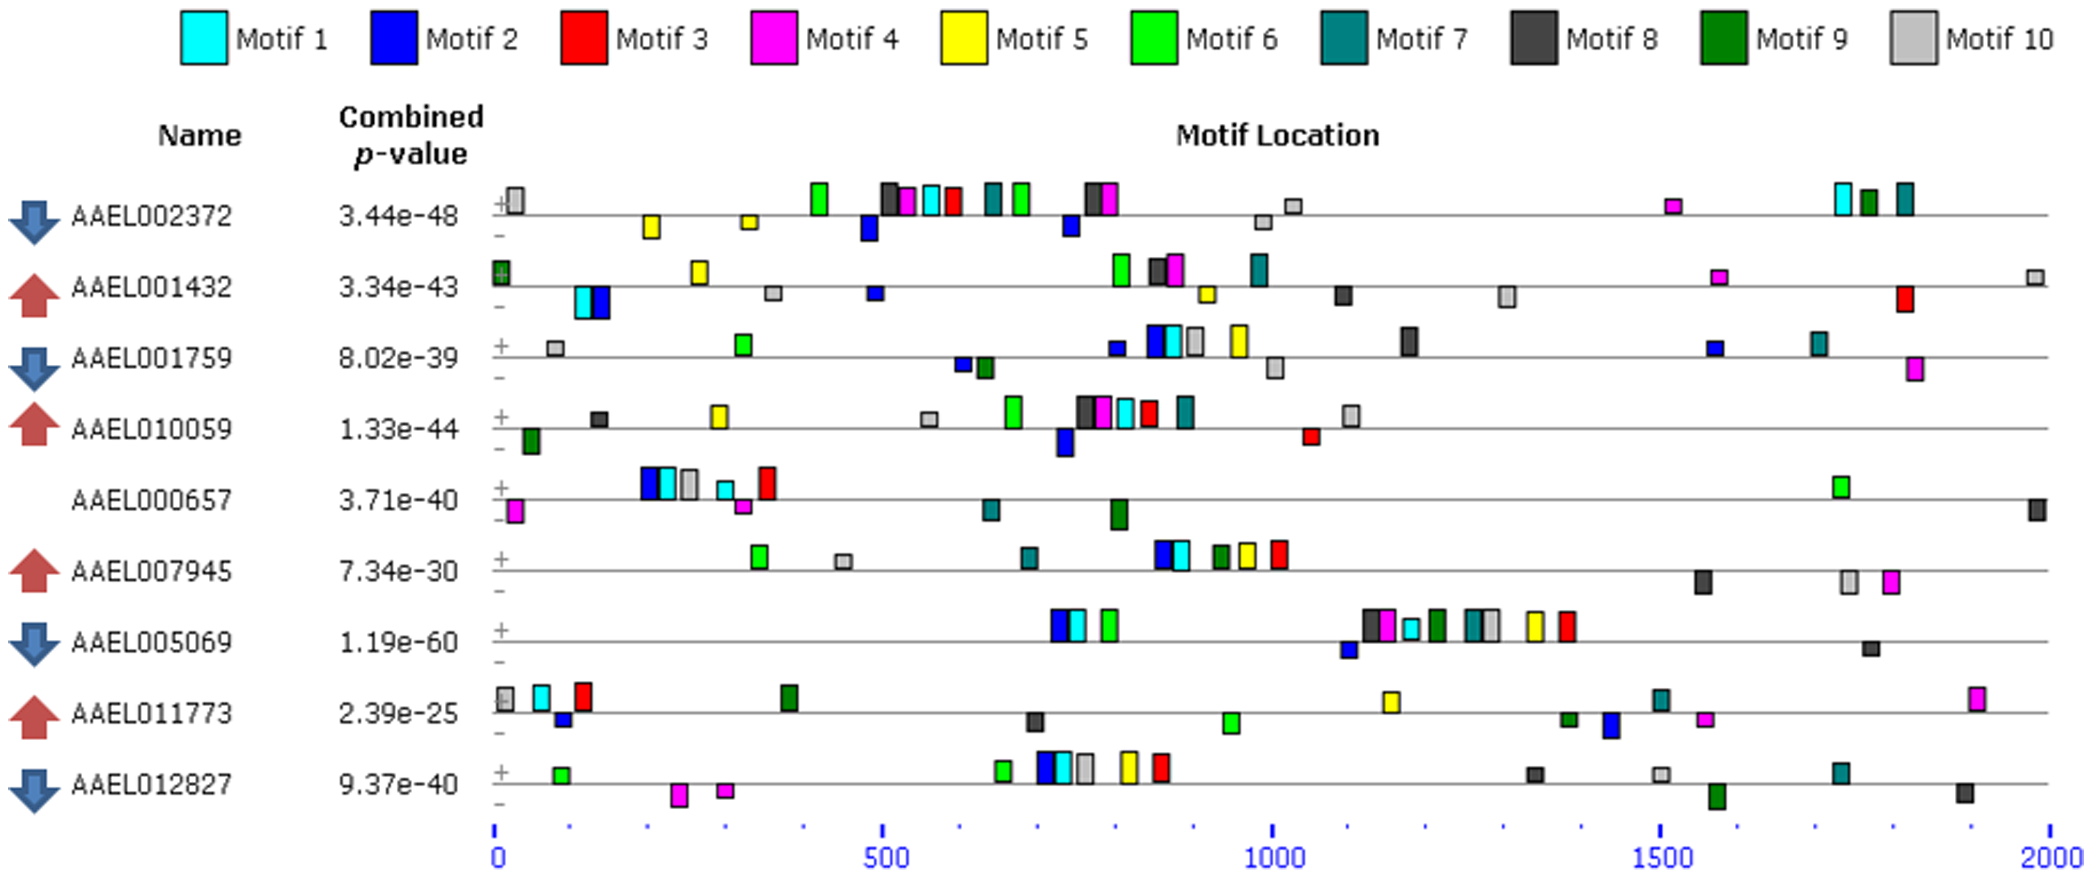
\includegraphics[width=.99\textwidth]{figures/figs/bonizzoni2012complex-cre.png}

\caption[MEME analysis of nine genes with \texorpdfstring{FPKM\textsubscript{DENVI}}{FPKM DENVI} ≥ 100 in carcasses and salivary glands at 14 dpi]{\sf \textbf{MEME analysis of nine genes with \texorpdfstring{FPKM\textsubscript{DENVI}}{FPKM DENVI} ≥ 100 in carcasses and salivary glands at 14 dpi} These genes also were identified with transcripts exhibiting significant differential accumulation in analyses of salivary gland samples of the Liverpool strain infected with DEV2 Thailand 16881 [26]. Colored boxes represent individual putative CREs and their locations in promoters of each gene. Red and blue arrows adjacent to Ensembl Gene ID indicate those genes whose transcripts were detected previously as more or less abundant following DENV infection [26]. Distances in base-pairs are provided below the schematic of each gene.
doi:10.1371/journal.pone.0050512.g004

Excerpted from \cite{bonizzoni2012complex}}
\label{fig:bonizzoni2012complex-cre}
\end{figure}

% \texorpdfstring{FPKM\textsubscript{DENVI}}{FPKM DENVI}

A total of 94 genes had FPKM ≥ 100 in \gls{DENVI} mosquitoes in both carcass and salivary gland samples at 14 \gls{dpi}, with corresponding values in B mosquitoes ≤ 100.
The putative promoter regions of these genes analyzed by MEME revealed the presence of two groups of motifs (Figure \ref{fig:bon2012complex-S5}: motifs 1, 2, 3, 4, 5, 7, 9, 10) co-occurring or alternating in 14 genes associated with diverse functions: AAEL001759 [40S ribosomal protein S9], AAEL005069 [ras-related protein Rab-1A], AAEL002372 [40S ribosomal protein S11], AAEL005165 [chaperone protein DNAj], AAEL000657 [hypothetical protein], AAEL005471 [Sec61 protein complex gamma subunit], AAEL001432 [protein disulfide isomerase], AAEL010059 [bacterial-type ABC transport ATP-binding subunit or RNAse l inhibitor], AAEL013407 [Catalase], AAEL007945 [eIF3 h], AAEL010169 [hypothetical protein], AAEL012827 [endoplasmin], AAEL011773 [calreticulin], AAEL010777 [TRX, putative].
These genes, except for AAEL002372, had high read coverage also in midgut samples, but not necessarily higher or equal accumulation in \gls{DENVI} versus B mosquitoes.
Some of these genes were detected previously as significantly differentially accumulated in the salivary glands of mosquitoes of the Liverpool strain (LVP) infected with \gls{DENV}2 Thailand 16681 (Figure \ref{fig:bonizzoni2012complex-cre}; \cite{Luplertlop2011}).
Specifically, the transcription products of AAEL001432, AAEL010059, AAEL007945 and AAEL011773 were more abundant in salivary glands of infected LVP, while the opposite was observed for AAEL001759, AAEL005069, AAEL002372 and AAEL012827, which were more abundant in uninfected samples.
AAEL00657 was listed as both up- and down-regulated following \gls{DENV} infection, most likely at different time points, but this is not explicit in the report \cite{Luplertlop2011}.
MADS\_MCM1+SFF\_M01051 and bZIP transcription factors were the best matches to motifs 1, 2, 5 and 7 (e-value ≤ $E-5$).
Motif 3 has sequence similarity with motifs 5 and 7 of the previously designated “carcass module” and matches to trp\_AtMYB-84\_M00970 (e-value = $2.25E-10$) and RREB-1 (e-value = $2.16E-7$).
The best match of motif 9 is to the HMG transcription factor ($1.87E-5$).


\subsection{Discussion}

The dengue-susceptible strain \gls{CTM} is well-documented in its ability to disseminate quickly viruses to peripheral tissues when compared to long-established laboratory strains \cite{Salazar2007}.
We describe in \citet{bonizzoni2012complex} changes in transcript accumulation levels in \gls{CTM} during the course of a Jam 1409 \gls{DENV}2 infection.
Our analyses include multiple post-infection time-points and three tissues important for the viral transmission cycle: midguts, salivary glands and carcasses, the latter of which includes the fat body.
The RNA-seq technology used in this study interrogates the whole \Aa\ transcriptome and allows for absolute quantification of poly-adenylated RNA levels.
In general, more depleted rather than enriched transcript accumulation was observed.
Importantly, hundreds of genes had exclusive read-coverage only in \gls{DENVI} mosquitoes, but their accumulation levels were generally low (FPKM$_{DENVI}$ < 4 in carcass and midgut samples and < 15 in salivary gland samples).

The “\gls{DENV} down-regulation” trend is consistent to that observed with the Rockefeller (ROCK) strain infected by \gls{DENV}2 New Guinea in transcriptional responses examined in whole-body (1–2, 7 and 14 \gls{dpi}) or midgut samples (10 \gls{dpi}) and in salivary glands of the LVP strain infected with \gls{DENV}2 Thailand 16681 \cite{Xi2008}, \cite{Luplertlop2011}, \cite{Sim2012}, \cite{Colpitts2011}.
These results support the hypothesis that dengue infection has a negative impact on fitness.
However, a larger number of genes had products that increased instead of decreased in abundance in carcass samples 10 \gls{dpi} and in salivary glands at 14 \gls{dpi} in ROCK mosquitoes infected with \gls{DENV}2-New Guinea \cite{Xi2008}, \cite{Sim2012}.
This trend also was evident in \Aa\ Aag2 cultured cells infected by \gls{DENV}2 New Guinea and in both susceptible (Moyo-S) and resistant (Moyo-R) strains infected with \gls{DENV}2 Jam1409 \cite{Sim2010}, \cite{Behura2011}.
These results emphasize the complex relationship among \Aa\ and dengue viruses.



\subsubsection{\textit{Cis}-regulatory Elements}

The preferred promoter for an anti-dengue effector gene would be one that is induced following a bloodmeal and is not affected by viral infection.
Furthermore, we hypothesize that genes with this preferred expression profile may share common regulatory mechanisms based on common \glspl{CRE}.
\alert{Analysis of the 5′-end of genes whose transcripts exhibited accumulation profiles exclusively in salivary gland following \gls{DENV} infection did not reveal conservation of \glspl{CRE}.
The regulation of these genes is likely not coordinated through common promoter elements. [point trying to make]}
In contrast, putative \glspl{CRE} were identified for genes whose transcripts were represented and modulated highly in response to dengue infection in midguts (1–4 \gls{dpi}), carcasses (all time points studied) and salivary glands and carcasses (14 \gls{dpi}).

Several of the identified motifs showed high-quality matches to known transcription factors.
The \glspl{CRE} likely are not related specifically to dengue infection since the majority of the genes included in the analyses also had read coverage in B mosquitoes.
This observation does not affect the potential utility of the \glspl{CRE} as components of synthetic promoters to direct expression of anti-dengue effector molecules.
Indeed, driving effector gene expression with control DNA that responds to an uninfected bloodmeal and either is unaffected or is enhanced by an infected bloodmeal could elicit a protective antiviral response in the mosquitoes.
Remarkably, 10 genes whose transcripts were modulated following \gls{DENV}2 16881 infection in LVP salivary gland samples were among the 14 genes with FPKM$_{DENVI}$ ≥ 100 in our carcass and salivary gland samples that have a common group of \gls{CRE} motifs \cite{Luplertlop2011}.
However, not all of these ten genes had transcripts that were consistently more abundant following infection, and one gene, (AAEL00657), had transcripts reported as more and less abundant \cite{Luplertlop2011}.
These results and the findings that several motifs are putative binding sites for transcription factors acting through repressors and activators support a complex model of transcription modulation that requires further investigation.

\subsection{Conclusions}

The study of genome-wide changes in transcript abundance in \Aa\ following dengue infection is anticipated to identify genes and control DNA elements involved in vector competence.
This knowledge is expected to contribute to development of novel vector control strategies.
The interactions between the mosquito host and the virus are complex at both the individual and population levels.
Many mosquito tissues are affected by the virus during the course of the infection and \Aa\ strains can show unique responses of the transcriptome in response to a blood meal and susceptibility to \gls{DENV} infection \cite{Black2002}, \cite{bonizzoni2012strain}.
Additionally, the variation in \gls{DENV} serotypes and genotypes contributes to genetically-distinct differences in vector competence \cite{Anderson2006}, \cite{Weaver2009}.
While we identified modulations in transcript abundance following \gls{DENV} infection that represent genes encoding similar functional categories, a limited number of specific genes were concordant across the mosquito strains and \gls{DENV}2 genotypes following comparison of our data with previous studies \cite{Xi2008}, \cite{Luplertlop2011}, \cite{Behura2011}, \cite{Sim2012}, \cite{Colpitts2011}.
Furthermore, the direction of changes in transcript abundance in samples from infected and uninfected mosquitoes was not always conserved among the various studies, an observation that we consider independent of the methodology used to assess differential transcript accumulation.
These results support the need for a comprehensive analysis of dengue infection focusing on recently-colonized laboratory strains or wild-caught mosquitoes to capture most of the genetic variability at the host level and different \gls{DENV} serotypes/genotypes \cite{Armstrong2001}.
This analysis also should account for possible variation in the progression of the viral infection and timing of host gene expression.